%# -*- coding: utf-8-unix -*-
%%==================================================
\chapter{Redis}
\label{chap1}
\begin{itemize}[noitemsep,topsep=0pt,parsep=0pt,partopsep=0pt]
	\item ...
\end{itemize}

\section{知识点和方法论}

\subsubsection{布隆过滤器}

原理: 简单的说就是, 有一个长的二进制数组, 然后, 通过多个hash函数映射到上面, 如果某个key没有映射到已经被映射的数组bit位上我们就认为这个数不存在. 如果已经映射了, 我们就认为这个数存在. 但是这有一定的概率失败. 如果hash函数都映射到已经映射的位置上, 所以有一定的误判率.

可以简单使用google的布隆过滤器, 简单的说就是在某些场景下, hashmap的性能消耗过多. 不适合做. 可以简单解决缓存穿透的问题. 即, 不存在的对象进行数据库访问我们可以用布隆过滤器进行拦截.

\subsubsection{如何解决并发数据一致性问题?}
1. 使用分布式锁

2. 使用mysql悲观锁 for update, 行锁, 加上排它锁, 这样后来的事物会阻塞查询, 这样就比变了数据不一致.

3. 使用mysql乐观锁, 基于CAS 当我心中预想的金额或者版本等于我想要的版本的时候更新整个账户金额

Update t\_account set money=\#{new\_money} where id=\#{id} and money=\#{old\_money};
\subsubsection{Redis的数据结构及使用场景}
字符串(string), 用来缓存简单的数据结构, 简单的字符串, 可以实现Session共享\par
列表(list), Redis的列表通过命令的组合, 即可以当做栈, 也可以当做队列来使用\par
集合(set), 可以实现自己和某人共同关注的人\par
散列表(hash), 存储一些key-value对, 更适合用来存储对象\par
有序集合(sorted set). 设置顺序, 实现排行榜的功能\par
\subsubsection{Redis集群策略}
一主多从, 整个集群所能存储的数据收到某台机器的内存容量, 所以不可能支持特大数据量, 一般加上哨兵模式来使用 \par

优点:

哨兵模式是基于主从模式的,所有主从的优点,哨兵模式都具有。
当某个master服务下线时,自动将该master下的某个从服务升级为master服务替代已下线的master服务继续处理请求sentinal与redis1和redis2建立长连接,与主机连接是心跳机制,

主从可以自动切换,系统更健壮,可用性更高。

缺点:

Redis较难支持在线扩容,在集群容量达到上限时在线扩容会变得很复杂。
\begin{figure}
	\centering
	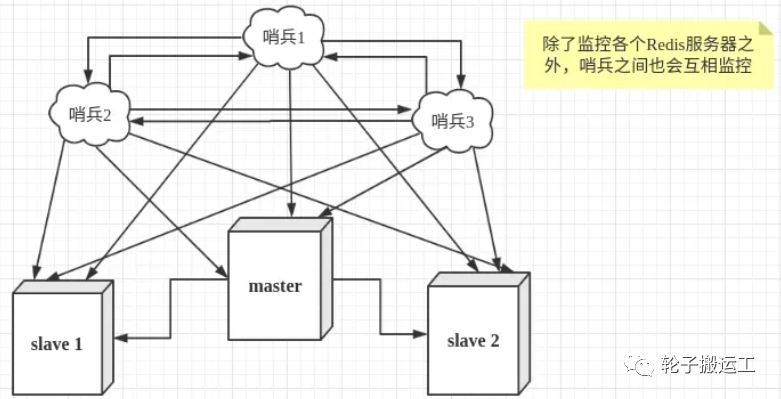
\includegraphics[width=0.7\linewidth]{figures/redis_sentinel.png}
	\caption{redissentinel}
	\label{fig:redissentinel}
\end{figure}

Cluster模式: 槽分配. 支持多主多从
为了保证高可用,redis-cluster集群引入了主从模式,一个主节点对应一个或者多个从节点,当主节点宕机的时候,就会启用从节点。当其它主节点ping一个主节点A时,如果半数以上的主节点与A通信超时,那么认为主节点A宕机了。如果主节点A和它的从节点A1都宕机了,那么该集群就无法再提供服务了。

当竞选从节点收到过半主节点同意,便会成为新的主节点。此时会以最新的Epoch通过PONG消息广播,让Redis Cluster的其他节点尽快的更新集群信息。当原主节点恢复加入后会降级为从节点。
\url{https://blog.csdn.net/zhibo_lv/article/details/105239297}
\begin{figure}
	\centering
	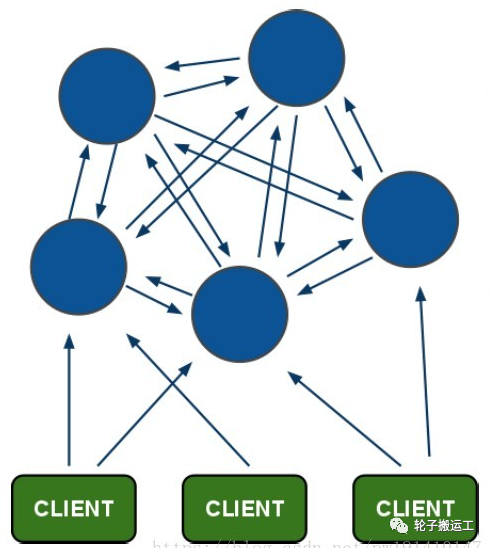
\includegraphics[width=0.7\linewidth]{figures/redis_cluster.png}
	\caption{rediscluster}
	\label{fig:rediscluster}
\end{figure}

\subsubsection{什么是Redis?}
\begin{enumerate}
	\item 高性能非关系型数据库
	\item 可以存储五种不同类型的额值之间的映射. 键的类型只能为字符串, 值支持五种类型数据:字符串(string), 列表(list), 集合(set), 散列表(hash), 有序集合(sorted set).
	\item redis数据是存在内存中的, 所以读写速度非常快.
\end{enumerate}
\subsubsection{简述Redis单线程模型?}
实现方式
\par
(1) I/O多路复用
\par
简单来说, 可以使用I/O多路复用来坚定多个socket连接, 然后将感兴趣的时间注册到内核中并监听每个事件是否发生.
\par
(2) 基于事件驱动
\par
服务器需要处理两类事件, 文件事件; 时间事件.
\par
当被监听的套接字准备好执行连接应答(accept), 读取(read), 写入(write), 关闭(close)等操作时, 与操作相对应的文件事件就会产生, 这时文件事件处理器就会调用套接字之前关联好的事件处理器来处理这些事件.
\par
文件事件处理器(file event handler) 主要包含4个部分: 多个socket(客户端链接), IO多路复用, 文件事件分派; 事件处理;
\begin{figure}
	\centering
	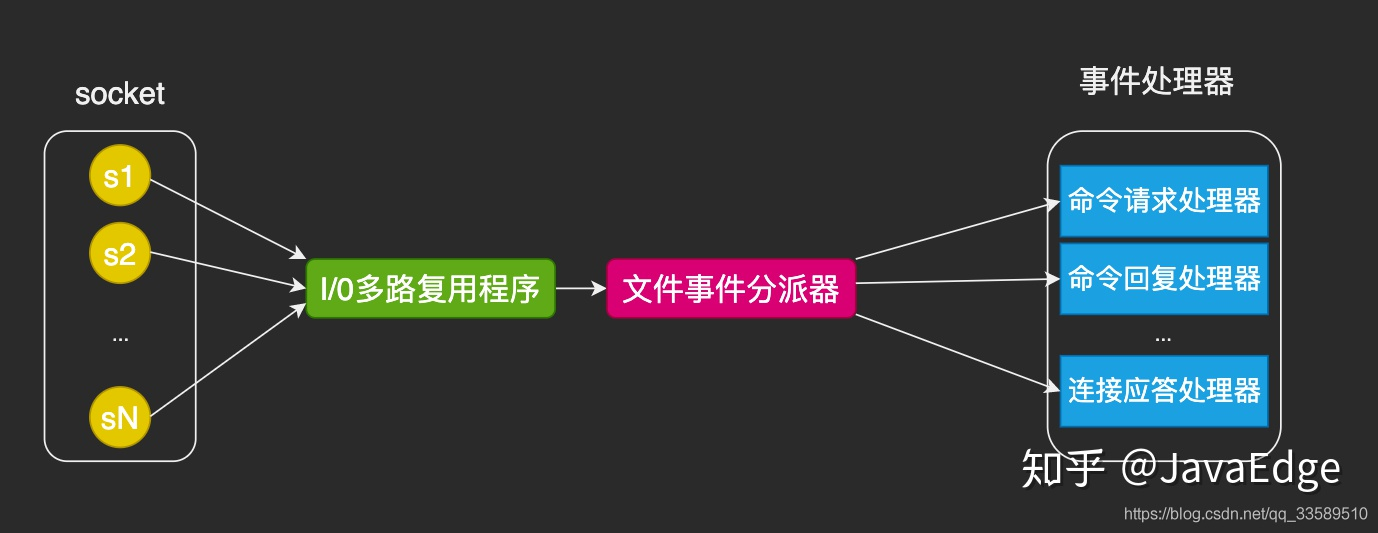
\includegraphics[width=0.7\linewidth]{figures/redis_file_event.jpg}
	\caption{redisfileevent}
	\label{fig:redis_file_event}
\end{figure}
\subsubsection{Redis五种类型数据的实现方式}
\begin{table}[!htbp]
	\centering
	\caption{实现}
	\begin{tabular}{|l|r|}

		\hline
		类型   & 编码                                                                \\
		\hline
		STRING & INT(整形, 在String中存储整形会是的)                                 \\
		\hline
		STRING & EMBSTR(简单动态字符串, 对于短小的string(44位字符)会使用这种结构)    \\
		\hline
		STRING & RAW(简单动态字符串, 对于稍微长一点的string会使用(44位字符)这种结构) \\
		\hline
		LIST   & QUICKLIST(快表)                                                     \\
		\hline
		LIST   & LINKEDLIST(快表)                                                    \\
		\hline
		SET    & INTSET(整数集合)                                                    \\
		\hline
		SET    & HT(哈希表)                                                          \\
		\hline
		ZSET   & ZIPLIST(压缩列表)                                                   \\
		\hline
		ZSET   & SKIPLIST(跳表)                                                      \\
		\hline
		HASH   & ZIPLIST(压缩列表)                                                   \\
		\hline
		HASH   & HT(哈希表)                                                          \\
		\hline
	\end{tabular}
\end{table}
字符串结构SDS和C中char[]有什么不同
\begin{enumerate}
	\item 获取SDS中字符串的长度因为SDS中存储了字符串的长度len属性, 直接访问, 时间复杂度O(1), 对于C语言获取字符串的长度需要经过遍历, 时间复杂度O(n).
	\item 避免缓冲区溢出, 会检查SDS中属性, free(空闲空间)能够实现字符串的扩充判断. 不足会重新申请空间.
	\item SDS支持空间预分配, 扩展的内存比实际需要的多
	\item SDS支持空间惰性释放, 字符串缩短之后, 不立即进行空间回收操作. SDS也提供相应API, 可以对冗余空间进行回收.
	\item 可以存储二进制, 因为SDS不以回车符号进行终止的判定.
\end{enumerate}
\subsubsection{redis字典的底层实现hashTable相关问题}
\begin{enumerate}
	\item 解决冲突: 链地址法, 即使用数组+链表的方式实现.
	\item 扩容: 有两个指针h[0] 和 h[1], h[1] 用来备份, 当h[0], 满了使用渐进值hash, 插入都插入h[1], 查找两个表都进行查找.
\end{enumerate}
\subsubsection{压缩链表原理ziplist}
连续内存, 包含多个节点entry.
\begin{figure}
	\centering
	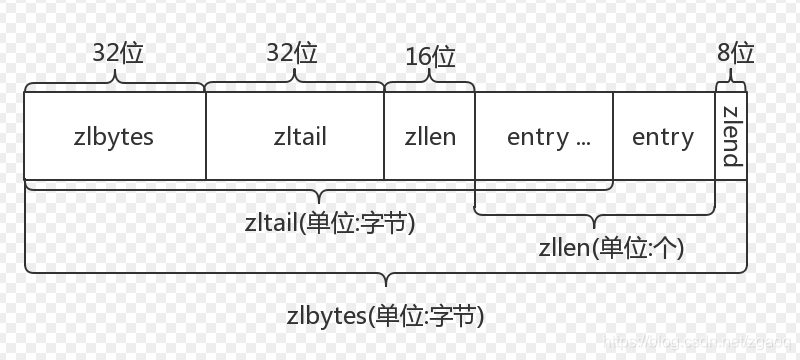
\includegraphics[width=0.7\linewidth]{figures/ziplist.png}
	\caption{ziplist}
	\label{fig:ziplist}
\end{figure}
\subsubsection{zset}
本质是舵机链表并有序.
skiplist与平衡树, 哈希表的比较
\begin{enumerate}
	\item skiplist和各种平衡树的元素排序是有序 的, 而哈希表不是有序的, 因此, 在哈希表上智能做单个key的查找, 不适宜做范围查找.
	\item 在做范围查找的时候, 平衡树比skiplist操作要复杂. 在平衡树上, 需要做一步回退操作. 而在skiplist上进行范围查找就非常简单, 只要找到最小值之后对第一层链表进行若干部遍历就可以实现.
	\item 平衡树插入和删除操作, 会引起结构调整, 操作复杂, skiplist的插入和删除只需要修改相邻节点的指针, 操作简单又快速.
\end{enumerate}

\subsubsection{AOF和RDB两种持久化方式区别}
\begin{enumerate}
	\item AOF存储命令, RDB存储数据.
	\item AOF文件因为存储命令, 所以在redis启动的时候加载aof会比加载rdb要慢.
	\item Redis 4.0 之后 启动了混合模式, AOF不需要是全量日志, 只要保存前一次RDB存储开始到这段时间增量AOF日志即可.
\end{enumerate}
\subsubsection{Redis中过期策略和缓存淘汰机制}
\begin{enumerate}
	\item 定期删除: redis默认每隔100ms随机对key检查, 有过期的key则进行删除. 容易导致很多过期的key没被发现
	\item 惰性删除: 获取某个key的时候, redis会检查一下, 如果过期了就进行删除.
\end{enumerate}
\subsubsection{为什么要使用Redis}
\begin{enumerate}
	\item 高性能: 内存的读取比硬盘乃至固态硬盘的读取速度都要快得多
	\item 高并发: 直接操作缓存能够承受的请求是远远大于直接访问数据库的, 所以我们可以考虑把数据库中的部分数据转移到缓存中去, 这样用户的一部分请求会直接请求缓存这里而不用经过数据库.
	\item 高性能: 使用多路I/O复用木星, 非阻塞IO;
\end{enumerate}
\subsubsection{Redis底层实现跳表介绍一下}
跳表是带多级索引的链表, 时间复杂度O(lgn), 所能实现的功能和红黑树差不多, 但是跳表有一个区间查找的优势, 红黑树没有.
\begin{figure}
	\centering
	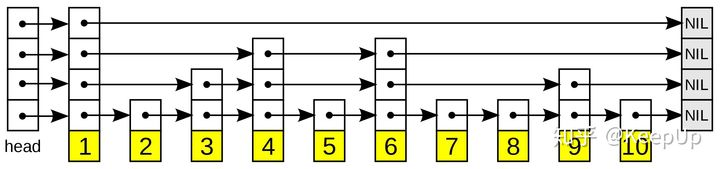
\includegraphics[width=0.7\linewidth]{figures/jump_table.jpg}
	\caption{jumptable}
	\label{fig:jumptable}
\end{figure}
\begin{enumerate}
	\item 表头: 负责维护跳表的节点指针.
	\item 跳跃表节点: 保存着元素值, 以及多个层.
	\item 层: 保存着指向其他元素的指针, 高层的指针越过的元素数量大于等于底层的指针, 为了提高查找效率, 程序总是从高层先开始访问, 然后随着元素值范围的缩小, 慢慢降低层次.
	\item 表尾: 全部由NULL组成.
\end{enumerate}

\subsubsection{为什么要使用Redis而不用map/guavaCache做缓存}
\begin{enumerate}
	\item guavaCache实现的是本地缓存, 最主要的特点是轻量化以及快速, 生命周期随着jvm的销毁而结束, 并且在多实例的情况下, 每个实例都需要个字保存一份缓存, 缓存容易出现不一致性.
	\item 使用redis之类的缓存称为分布式缓存, 在多实例的情况下, 各实例公用一份缓存数据, 缓存具有一致性.
\end{enumerate}
\subsubsection{分布式锁如何使用redis实现}
\begin{enumerate}
	\item setnx命令原子性实现.
\end{enumerate}
\subsubsection{Redis的内存淘汰策略有哪些}
Redis的内存淘汰策略是指在Redis用于缓存的内存不足时, 怎么处理需要新写入且需要申额外空间的数据.
全局的键空间选择性移除
\begin{enumerate}

	\item noeviction: 当内存不足以容纳新写入数据时, 新写入操作会报错.
	\item allkeys-lru: 当内存不足以容纳新写入数据时, 在键空间中, 移除最近最少使用的key.
	\item allkeys-random: 当内存不足以容纳新写入数据时, 在键空间随机移除某个key.
\end{enumerate}
设置过期时间的键空间选择性移除
\begin{enumerate}

	\item volatile-lru: 当内存不足以容纳新写入数据时, 在设置了过期时间的键空间中, 移除最近最少使用的key.
	\item volatile-random: 当内存不足以容纳新写入数据时, 在设置了过期时间的键空间中, 随机移除某个key.
	\item volatile-ttl: 当内存不足以容纳新写入的数据时, 在设置了过期时间的键空间中, 有更早过期时间的key优先移除.
\end{enumerate}
\subsubsection{Redis事物的概念}
Redis事物的本质通过MULTI, EXEC, WATCH等一组命令的集合.
\begin{enumerate}

	\item 事物开始 MULTI
	\item 命令入队
	\item 事务执行 EXEC
\end{enumerate}
* 事务执行过程中, 如果服务端收到有EXEC, DISCARD, WATCH, MULTI之外的请求, 将会把请求放入队列中排队.
简单介绍一下watch, 当watch的变量在事务过程中发生了改变, 那么事务失败, 拒绝执行事物.
\begin{lstlisting}
	>watch 'name'
	>multi
	>set "name" "peter"
	>exec
	(nil)
\end{lstlisting}
\subsubsection{RedisSharding问题}
简单来说就是多个client 连接多个redis, 然后通过一致性哈希算法, 来确定访问的key+访问的客户端名字在哪一台redis上.
采用的算法是MURMUR\_HASH,
\begin{figure}
	\centering
	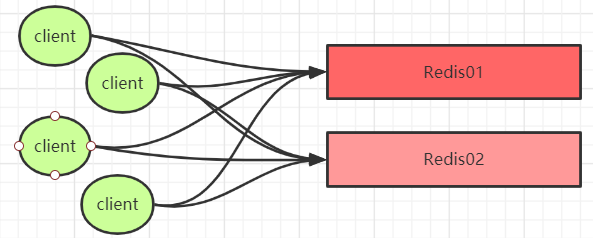
\includegraphics[width=0.7\linewidth]{figures/redis_sharding.png}
	\caption{redis\_sharding}
	\label{fig:redissharding}
\end{figure}
\subsubsection{缓存雪崩}
缓存同一时间大面积的失效, 所以, 后面的请求都会落到数据库上, 造成数据库短时间内承受大量请求而崩掉

\par
\textbf{解决方案}
\begin{enumerate}

	\item 缓存数据的过期时间设置随机, 防止同一时间大量数据过期现象发生.

\end{enumerate}

\subsubsection{缓存穿透}
缓存和数据库中都没有数据, 导致所有的请求都落在数据库中, 造成数据库短时间内承受大量请求而崩掉.
\par
\textbf{解决方案}
\begin{enumerate}

	\item 从缓存中取不到的数据, 在数据库中也没有取到, 这时也可以将key-value对写为key-null, 缓存时间设定为30s.

\end{enumerate}

\subsubsection{缓存击穿}
缓存中没有但数据库中有的数据, 由于并发用户特别多, 同时读缓存没读到数据, 又同时去数据库取数据, 引起数据库压力瞬间增大, 造成过大压力, 和缓存雪崩不同的是, 缓存击穿指并发查询同一条数据, 缓存雪崩是不同数据都过期了, 很多数据都查不到, 从而查数据库.
\par
\textbf{解决方案}
\begin{enumerate}
	\item 设置热点数据永不过期
\end{enumerate}
\subsubsection{缓存预热}
系统上线后, 将相关的缓存数据直接加载到缓存系统. 这样就可以避免在用户请求的时候, 先查询数据库, 然后再讲数据缓存的问题, 用户直接查询事先被预热的缓存数据.
\par
\textbf{解决方案}
\begin{enumerate}
	\item 定时刷新缓存;
\end{enumerate}
\subsubsection{Redis6.0 为什么要引入多线程呢?}
Redis将所有数据放在内存中, 内存的相应市场大约100ns, 对于小数据包, Redis服务器可以处理8w到10wQPS, 这也是Redis处理的极限了, 对于80\%的公司来说, 单线程的redis已经足够使用了.
\par
但随着越来越复杂的业务场景, 需要更大的QPS.
\begin{enumerate}
	\item 可以充分利用服务器CPU资源, 目前主线程只能利用一个核
	\item 多线程任务可以分摊Redis同步IO读写负荷.
\end{enumerate}
\subsubsection{Redis主从复制模式}
\begin{enumerate}
	\item 完全同步:刚开始, 主服务器发送RDB文件给从服务器, 实现主从同步.
	\item 部分同步:当连接由于网络原因断开的时候, 将中间断开的执行的写命令发送给从服务器. 实现同步.
\end{enumerate}

\begin{figure}
	\centering
	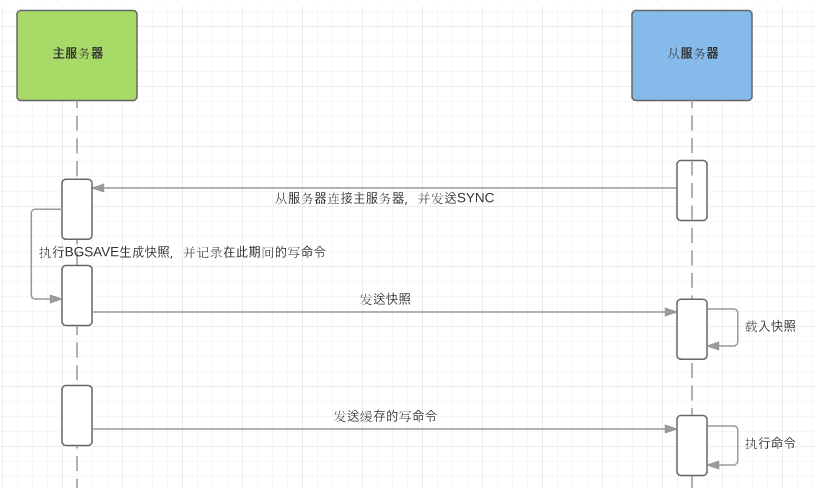
\includegraphics[width=0.7\linewidth]{figures/redismasterslave.png}
	\caption{redismasterslave}
	\label{fig:redismasterslave}
\end{figure}

简单来说, 从服务器发送SYNC信号给主服务器, 主服务将RDB快照发送给从服务器, 从服务器更新快照内容. 主服务器将缓存写命令发送给从服务器.

\subsubsection{Redis中持久化机制}
\begin{enumerate}
	\item
\end{enumerate}
